\begin{pastexam}[label={px:nchu-113-dsa-05}]{中興資工所甲組 113 學年度 選擇題第 5 題}
（單選；每題 2 分，答錯倒扣 0.5 分）

The following items are inserted into a \textbf{binary search tree}: 6, 3, 5, 2, 4, 7, 1, 9, 8. What is the
\textbf{sum} of the deepest node(s)?

(A)~14 \qquad (B)~12 \qquad (C)~4 \qquad (D)~8 \qquad (E)~None of the above.
\end{pastexam}

\begin{pastsoln}
答案是 (E)（最深的節點是 $1$、$4$、$8$，和是 $13$）。

依序插入（資結書第~9.2~節：從根往下比，小的往左、大的往右，走到空位就放）：
\begin{itemize}
\item $6$ 當根；$3 < 6$ 放左；$5$：$< 6$ 往左，$> 3$ 放 $3$ 的右邊；$2$：放 $3$ 的左邊；
\item $4$：$< 6$、$> 3$、$< 5$，放 $5$ 的左邊；$7 > 6$ 放根的右邊；$1$：放 $2$ 的左邊；
\item $9$：$> 6$、$> 7$，放 $7$ 的右邊；$8$：$> 6$、$> 7$、$< 9$，放 $9$ 的左邊。
\end{itemize}

\begin{center}
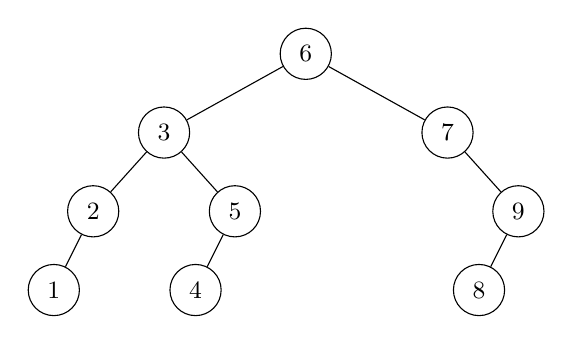
\begin{tikzpicture}[v/.style={circle,draw,minimum size=6.5mm,inner sep=1pt,font=\small},
  level distance=10mm, level 1/.style={sibling distance=36mm},
  level 2/.style={sibling distance=18mm}, level 3/.style={sibling distance=10mm}]
\node[v] {6}
  child {node[v] {3}
    child {node[v] {2} child {node[v] {1}} child[missing]}
    child {node[v] {5} child {node[v] {4}} child[missing]}}
  child {node[v] {7}
    child[missing]
    child {node[v] {9} child {node[v] {8}} child[missing]}};
\end{tikzpicture}
\end{center}

深度（根是 $0$）：$6$ 是 $0$；$3, 7$ 是 $1$；$2, 5, 9$ 是 $2$；$1, 4, 8$ 是 $3$。 最深的一層有三個節點，
和是 $1 + 4 + 8 = 13$，不在 (A)--(D) 裡，選 (E)。
\end{pastsoln}
